\documentclass[11pt,a4paper]{article}
\usepackage[utf8]{inputenc}
\usepackage[spanish,es-tabla]{babel}
\usepackage[margin=2.2cm]{geometry}
\usepackage{helvet}
\renewcommand{\familydefault}{\sfdefault}

% Packages for visual enhancement
\usepackage{amsmath}
\usepackage{xcolor}
\usepackage{tikz}
\usetikzlibrary{shapes.geometric, arrows.meta, positioning, shadows, babel}
\usepackage{pgfgantt}
\usepackage{booktabs}
\usepackage{tabularx}
\usepackage{array}
\usepackage{enumitem}
\usepackage{titlesec}
\usepackage{fancyhdr}
\usepackage{hyperref}
\usepackage{graphicx}
\usepackage{pdflscape}

% Define color palette
\definecolor{primary}{RGB}{37, 99, 235}     % Blue #2563EB
\definecolor{secondary}{RGB}{125, 211, 252} % Light Blue #7DD3FC
\definecolor{accent}{RGB}{34, 197, 94}      % Green #22C55E
\definecolor{darkbg}{RGB}{31, 41, 55}      % Dark Gray #1F2937
\definecolor{lightbg}{RGB}{243, 244, 246}   % Light Gray #F3F4F6
\definecolor{cardbg}{RGB}{248, 250, 252}

% Setup hyperref
\hypersetup{
	colorlinks=true,
	linkcolor=primary,
	filecolor=primary,      
	urlcolor=primary,
	pdftitle={Documento de Especificacion - Fase 1},
	pdfauthor={Elmer Wilson}
}

% Page style setup
\pagestyle{fancy}
\fancyhf{}
\setlength{\headheight}{15pt}
\lhead{\small \textcolor{gray}{Iglesia Getsemaní — Sistema Web de Finanzas e Inventario}}
\rhead{\small \textcolor{gray}{Fase 1: Especificación}}
\cfoot{\thepage}
\renewcommand{\headrulewidth}{0.4pt}
\renewcommand{\footrulewidth}{0.4pt}

% Section styling
\titleformat{\section}
{\color{primary}\normalfont\large\bfseries}
{\thesection.}{0.5em}{}[\titlerule]
\titleformat{\subsection}
{\color{darkbg}\normalfont\bfseries}
{\thesubsection}{0.5em}{}

\setlist[itemize]{noitemsep, topsep=3pt, leftmargin=*}
\setlist[enumerate]{noitemsep, topsep=3pt, leftmargin=*}
\usepackage{tikz}
\usetikzlibrary{shapes.geometric, arrows, positioning}
\begin{document}
	\shorthandoff{><}
	
	% --- PORTADA FORMAL ---
	\begin{titlepage}
		\centering
		\vspace*{1cm}
		
		{\Huge \bfseries \textcolor{primary}{DOCUMENTO DE ESPECIFICACIÓN}}\\[0.4cm]
		{\Large \bfseries \textcolor{darkbg}{FASE 1: ANÁLISIS, DISEÑO Y MODELADO}}\\[0.2cm]
		{\large \textcolor{gray}{Sistema Web de Finanzas e Inventario por Departamentos}}\\[1.5cm]
		
		\begin{tikzpicture}
			\node[
			draw=primary,
			fill=cardbg,
			line width=1.5pt,
			rounded corners=8pt,
			inner sep=15pt,
			text width=0.85\textwidth,
			align=center
			] {\Large \bfseries Iglesia Evangélica Getsemaní C.A, \\ Pueblo Nuevo Jucup, S.S. Coatán, Huehuetenango.};
		\end{tikzpicture}
		
		
		\vfill
		
		\begin{table}[h!]
			\centering
			\renewcommand{\arraystretch}{1.4}
			\begin{tabular}{p{5cm} p{8cm}}
				\toprule
				\textbf{Estudiante / Desarrollador:} & Elmer Wilson (Clave 13)  \\
				\textbf{Curso:} & Laboratorio de Seminario de Sistemas 1 \\
				\textbf{Fase entregada:} & Fase 1 — Análisis, Investigación y Diseño de Producto \\
				\textbf{Fecha de inicio del proyecto:} & 09 de agosto de 2026 \\
				\textbf{Fecha de entrega de esta fase:} & 18 de agosto de 2026 \\
				\bottomrule
			\end{tabular}
		\end{table}
		
		\vfill
		{\small Quetzaltenango, Guatemala \hfill Año 2026}
	\end{titlepage}
	
	\newpage
	\tableofcontents
	\newpage
	
	% --- 1. INTRODUCCIÓN ---
	\section{Introducción}
	Este documento constituye la entrega de la \textbf{Fase 1} del proyecto \emph{Sistema Web de Finanzas e Inventario por Departamentos}, desarrollado para la Iglesia Evangélica Getsemaní, ubicada en Pueblo Nuevo Jucup, S.S. Coatán, Huehuetenango, en el marco del curso de Laboratorio de Seminario de Sistemas 1. Su propósito es dejar establecida la base conceptual, funcional y de diseño sobre la cual se construirá el sistema en las fases 2 y 3, aplicando los enfoques de \textbf{BPM}, \textbf{ERP ligero}, \textbf{CRM básico}, \textbf{Cloud Computing} e \textbf{Ingeniería Agéntica} vistos en el curso.
	
	El contenido de este documento no se basa únicamente en la especificación verbal entregada por el cliente (Junta Directiva de la iglesia), sino también en el \textbf{análisis directo de los archivos operativos reales} que los tesoreros utilizan actualmente, lo cual permitió validar y enriquecer los requerimientos con la forma real de trabajo de la institución.
	
	% --- 2. MODELO DE NEGOCIO ---
	\section{Modelo de Negocio, Organigrama y Vocabulario Institucional}
	
	\subsection{Naturaleza del negocio}
	La Iglesia Evangélica Getsemaní no es una entidad con fines de lucro, por lo que el "modelo de negocio" del sistema se traduce en un \textbf{modelo de administración de recursos por centros de costo}, donde cada departamento, consejo, comité o congregación anexa administra su propio flujo de ingresos y egresos, pero rinde cuentas de forma consolidada ante la Junta Directiva y la Asamblea General.
	
	\subsection{Organigrama y flujo financiero}
	
	\begin{center}
		\begin{tikzpicture}[
			node distance=1.2cm and 0.8cm,
			box/.style={rectangle, draw=primary, fill=cardbg, rounded corners, align=center, font=\small, inner sep=6pt, line width=0.8pt},
			header/.style={rectangle, draw=primary, fill=primary, text=white, font=\small\bfseries, align=center, inner sep=5pt}
			]
			% Level 1
			\node[box] (ag) {\textbf{ASAMBLEA GENERAL}\\(Órgano Supremo Legal)};
			
			% Level 2
			\node[box, below=0.8cm of ag] (jd) {\textbf{JUNTA DIRECTIVA}\\Presidente $\cdot$ Vicepresidente $\cdot$ Secretario $\cdot$ Tesorero\\3 Vocales (Administra el sistema)};
			
			% Level 3
			\node[box, below left=1.2cm and 1.5cm of jd, text width=4cm] (c3) {\textbf{3 CONSEJOS PRINCIPALES}\\[2pt]\footnotesize Consejo Local (Diezmos/Ofrendas)\\Consejo Femenil\\Consejo Infantil};
			\node[box, below=1.2cm of jd, text width=4cm] (ca) {\textbf{COMITÉS AUTÓNOMOS}\\[2pt]\footnotesize Radio Estéreo Getsemaní\\Comité Infantil\\Comité Construcción};
			\node[box, below right=1.2cm and 1.5cm of jd, text width=4.2cm] (ca2) {\textbf{CONGREGACIONES ANEXAS}\\[2pt]\footnotesize Chamvacx (única que rinde cuentas dentro del sistema)};
			
			% Arrows
			\draw[thick, ->, >=stealth] (ag) -- node[right, font=\tiny] {Recibe Informe General} (jd);
			\draw[thick] (jd) -- ++(0,-0.6cm) -| (c3);
			\draw[thick] (jd) -- ++(0,-0.6cm) -- (ca);
			\draw[thick] (jd) -- ++(0,-0.6cm) -| (ca2);
		\end{tikzpicture}
	\end{center}
	
	Cada uno de estos grupos opera \textbf{como un mini-sistema contable independiente} (saldo propio, ingresos propios, egresos propios), pero todos alimentan la misma base de datos central, permitiendo la consolidación automática en el Informe General de Asamblea.
	
	\newpage
	
	\subsection{Vocabulario institucional}
	Para que el sistema sea familiar y natural para sus usuarios finales, se sustituye la terminología comercial estándar por el lenguaje propio de la institución:
	
	\begin{table}[h!]
		\centering
		\renewcommand{\arraystretch}{1.2}
		\begin{tabularx}{\textwidth}{l X}
			\toprule
			\textbf{Término técnico / comercial} & \textbf{Término institucional adoptado} \\
			\midrule
			Cliente / Usuario final & Hermano / Aportante \\
			Venta / Transacción de entrada & Ingreso (Diezmo, Ofrenda, Donación) \\
			Categoría de gasto & Nomenclatura / Cuenta de egreso \\
			Centro de costo & Departamento / Consejo / Comité \\
			Cierre contable & Corte de caja \\
			Consolidado financiero & Informe General de Asamblea \\
			Administrador del sistema & Tesorero Jurídico / Administrador General \\
			\bottomrule
		\end{tabularx}
	\end{table}
	
	% --- 3. MISIÓN, VISIÓN Y VALORES ---
	\section{Misión, Visión y Valores}
	
	\subsection{Misión y Visión de la Iglesia}
	\paragraph{Misión} Glorificar a Dios y proclamar el evangelio de Jesucristo, dando a conocer las buenas nuevas de salvación, promoviendo la enseñanza bíblica, la comunión, la oración y el servicio cristiano.
	
	\paragraph{Visión} Promover el desarrollo y madurez espiritual de los miembros, fomentando proyectos cristianos, educativos, culturales y de asistencia social, para impactar positivamente en la sociedad y cumplir con los fines de la Iglesia.
	
	\subsection{Misión y Visión del Software}
	\paragraph{Misión} Administrar con transparencia, fidelidad y orden los recursos financieros y bienes materiales encomendados a la Iglesia Evangélica Getsemaní, facilitando la rendición de cuentas de cada departamento ante la Junta Directiva y la Asamblea General.
	
	\paragraph{Visión} Ser un modelo de gestión administrativa eclesiástica respaldado por herramientas tecnológicas modernas, que automaticen los procesos financieros y de inventario, garantizando integridad de la información y agilidad en la preparación de asambleas.
	
	\subsection{Valores institucionales que guían el diseño del sistema}
	\begin{itemize}
		\item \textbf{Transparencia:} Todo movimiento debe quedar registrado y ser trazable.
		\item \textbf{Mayordomía:} Los recursos administrados no son propios, son encomendados; el sistema debe reflejar responsabilidad sobre cada aportación.
		\item \textbf{Integridad:} Ningún registro debe poder alterarse sin dejar evidencia (bitácora).
		\item \textbf{Orden:} Catálogos y nomenclaturas estandarizadas evitan la dispersión de criterios entre departamentos.
		\item \textbf{Servicio colaborativo:} Cada tesorero de departamento trabaja de forma autónoma, pero dentro de un marco común administrado centralmente.
	\end{itemize}

	\newpage
	% --- 4. PLANTEAMIENTO DEL PROBLEMA ---
	\section{Planteamiento del Problema}
	Actualmente, la tesorería de cada consejo, comité y congregación anexa lleva sus registros en hojas de cálculo independientes , las cuales luego son transcritas manualmente a un archivo consolidado  para su presentación en asambleas.
	
	Este proceso manual genera los siguientes problemas concretos:
	\begin{itemize}
		\item \textbf{Duplicidad de trabajo:} Los mismos datos se escriben primero en el libro del departamento y luego se vuelven a escribir en el consolidado anual.
		\item \textbf{Riesgo de descuadres:} El saldo final de un mes no siempre coincide con el saldo inicial declarado del siguiente, al depender de copiado manual.
		\item \textbf{Falta de trazabilidad:} No existe un registro de quién ingresó, modificó o eliminó un movimiento.
		\item \textbf{Lentitud en la rendición de cuentas:} Preparar el informe para la Asamblea Anual toma días de trabajo manual de consolidación.
		\item \textbf{Dependencia de un formato no estandarizado:} Cada tesorero puede nombrar las cuentas de forma distinta, dificultando comparar departamentos.
	\end{itemize}
	
	% --- 5. OBJETIVOS ---
	\section{Objetivos del Proyecto}
	
	\subsection{Objetivo General}
	Desarrollar una aplicación web ligera y ágil (tipo punto de venta simplificado, orientado a finanzas eclesiales) que permita registrar ingresos, egresos e inventarios por departamento, generando automáticamente los cortes de caja y el informe consolidado de asamblea que hoy se elaboran manualmente en Excel.
	
	\subsection{Objetivos Específicos}
	\begin{enumerate}
		\item Sustituir la captura manual en Excel por un \textbf{registro transaccional de movimientos} (ingresos/egresos) que alimente reportes de forma automática, en lugar de guardar reportes ya calculados.
		\item Implementar un esquema de \textbf{roles y permisos (RBAC)} que aísle la información de cada departamento, salvo para el Administrador General.
		\item Estandarizar los \textbf{catálogos de nomenclaturas} de ingresos y egresos, extraídos del análisis de los archivos reales de la iglesia.
		\item Automatizar el \textbf{cálculo de saldos} (inicial, movimientos, final) por departamento y periodo.
		\item Generar el \textbf{Informe General de Asamblea} consolidando automáticamente los 3 Consejos, los Comités Autónomos y la Congregación Chamvacx.
		\item Dejar preparada la arquitectura para incorporar, en fases posteriores, un \textbf{padrón de miembros/aportantes} y comprobantes en PDF.
	\end{enumerate}
	
	% --- 6. ALCANCE ---
	\section{Alcance del Proyecto}
	
	\subsection{Dentro del alcance}
	\begin{itemize}
		\item Registro de ingresos, clasificados por cuenta, con opción de identificar al aportante (CUI/DPI) o registrarlo como anónimo.
		\item Registro de egresos, clasificados por nomenclatura/código corto, con descripción, fecha y departamento responsable.
		\item Administración dinámica de departamentos, consejos, comités y congregaciones.
		\item Mantenimiento administrable de catálogos de cuentas.
		\item Cálculo automático de saldo de caja por departamento.
		\item Cortes de caja por periodo (diario, mensual, anual, personalizado).
		\item Informe General consolidado para Asamblea.
		\item Módulo básico de inventario de bienes por departamento (correcto, dañado, perdido).
		\item Bitácora de auditoría de creación, edición y eliminación de registros.
		\item Gestión de usuarios y roles RBAC.
	\end{itemize}
	
	\subsection{Fuera del alcance (fase 1–3)}
	\begin{itemize}
		\item Facturación electrónica tributaria (SAT / FEL).
		\item Integración con pasarelas de pago o cobro con tarjeta.
		\item Módulo de nómina/planillas con cálculos legales de retenciones.
		\item Aplicación móvil nativa.
		\item CRM completo de miembros con control de asistencia.
	\end{itemize}
	

	% --- 7. ANÁLISIS ECONÓMICO Y DE RIESGOS ---
	\section{Análisis Económico y de Riesgos}
	
	\subsection{Estimación económica}
	\begin{table}[h!]
		\centering
		\renewcommand{\arraystretch}{1.2}
		\begin{tabularx}{\textwidth}{X r}
			\toprule
			\textbf{Concepto} & \textbf{Estimado} \\
			\midrule
			Hosting de base de datos en la nube (capa gratuita, Fase 1–2) & \$0 USD/mes \\
			Hosting de base de datos en la nube (uso productivo, Fase 3 en adelante) & \$5–\$10 USD/mes aprox. \\
			Dominio web (opcional) & \$10–\$15 USD/año \\
			Certificado SSL & Incluido (gratuito) \\
			\bottomrule
		\end{tabularx}
	\end{table}
	
	\subsection{Riesgos identificados}
	\begin{table}[h!]
		\centering
		\renewcommand{\arraystretch}{1.2}
		\begin{tabularx}{\textwidth}{p{4.5cm} p{2.5cm} X}
			\toprule
			\textbf{Riesgo} & \textbf{Impacto} & \textbf{Mitigación} \\
			\midrule
			Resistencia al cambio & Medio-Alto & Interfaz simple, captura rápida por código y capacitación inicial. \\
			Pérdida de conexión a internet & Medio & Interfaz ligera optimizada para bajo consumo de datos. \\
			Errores de digitación en montos & Medio & Validaciones de formato y confirmación visual antes de guardar. \\
			Modificación indebida de registros & Alto & Cortes de caja congelados + bitácora de auditoría obligatoria. \\
			Proyecto individual & Medio & Documentación técnica exhaustiva y uso de GitFlow. \\
			\bottomrule
		\end{tabularx}
	\end{table}
	
	
	\newpage
	% --- 8. ESPECIFICACIÓN DE REQUERIMIENTOS ---
	\section{Especificación de Requerimientos}
	
	\subsection{Requisitos Funcionales (RF)}
	\begin{table}[h!]
		\centering
		\renewcommand{\arraystretch}{1.1}
		\begin{tabularx}{\textwidth}{l X}
			\toprule
			\textbf{Código} & \textbf{Descripción} \\
			\midrule
			RF-01 & Registrar ingresos con tipo, monto, fecha, departamento y aportante (opcional). \\
			RF-02 & Registrar egresos con nomenclatura/código, monto, fecha, descripción y departamento. \\
			RF-03 & Búsqueda rápida de cuentas de ingreso/egreso por código corto o nombre con autocompletado. \\
			RF-04 & Calcular saldo de caja en tiempo real: $\text{Saldo Final} = \text{Saldo Inicial} + \sum \text{Ingresos} - \sum \text{Egresos}$. \\
			RF-05 & Cortes de caja por periodo, evitando modificaciones retroactivas sobre periodos cerrados. \\
			RF-06 & Reporte por departamento con desglose de ingresos, egresos y balance neto. \\
			RF-07 & Informe General consolidado (3 Consejos, Comités Autónomos, Congregación Chamvacx). \\
			RF-08 & Exportar reportes generados a PDF y Excel. \\
			RF-09 & Registrar bienes de inventario (asociados a departamento; estado: Correcto, Dañado, Perdido). \\
			RF-10 & Mantenimiento administrable de departamentos, consejos, comités y congregaciones. \\
			RF-11 & Mantenimiento administrable de nomenclaturas de ingresos y egresos. \\
			RF-12 & Bitácora de auditoría (usuario, fecha/hora, acción realizada sobre cualquier registro). \\
			RF-13 & Gestión de usuarios y asignación de rol/departamento por el Administrador General. \\
			RF-14 & Padrón básico de aportantes/miembros (nombre, CUI/DPI) para trazabilidad. \\
			\bottomrule
		\end{tabularx}
	\end{table}
	
	\subsection{Requisitos No Funcionales (RNF)}
	\begin{table}[h!]
		\centering
		\renewcommand{\arraystretch}{1.1}
		\begin{tabularx}{\textwidth}{l X}
			\toprule
			\textbf{Código} & \textbf{Descripción} \\
			\midrule
			RNF-01 & Almacenamiento seguro de contraseñas (hash Bcrypt) y sesiones seguras de Laravel. \\
			RNF-02 & Base de datos alojada en proveedor Cloud/Serverless. \\
			RNF-03 & Tiempo de respuesta menor a 2 segundos en consultas y reportes estándar. \\
			RNF-04 & Interfaz responsive utilizable en PC y dispositivos móviles. \\
			RNF-05 & Aislamiento de datos por \texttt{departamento\_id} para usuarios tipo Tesorero. \\
			RNF-06 & Alta disponibilidad acorde a la capa de infraestructura cloud elegida. \\
			RNF-07 & Flujo de control de versiones GitFlow sin commits directos a \texttt{main}. \\
			\bottomrule
		\end{tabularx}
	\end{table}
	
	\newpage
	% --- 9. ROLES Y MATRIZ DE PERMISOS ---
	\section{Roles y Matriz de Permisos (RBAC)}
	
	\paragraph{Administrador General / Tesorero Jurídico:} Acceso total al sistema; crea y gestiona usuarios de cada departamento; asigna permisos granulares; visualiza y consolida reportes globales de todos los departamentos; aprueba cortes de caja.
	
	\paragraph{Contador / Tesorero de Departamento:} Acceso restringido a su departamento asignado; registra ingresos y egresos diarios/mensuales; puede modificar registros solo antes del corte de caja.
	
	\begin{table}[h!]
		\centering
		\renewcommand{\arraystretch}{1.2}
		\begin{tabularx}{\textwidth}{X c c}
			\toprule
			\textbf{Módulo / Función} & \textbf{Administrador General} & \textbf{Tesorero de Departamento} \\
			\midrule
			Gestión de usuarios y roles & Crear, modificar, desactivar & Sin acceso \\
			Mantenimiento de catálogos & Crear y editar & Solo lectura \\
			Registro de ingresos/egresos & Todos los departamentos & Solo su departamento \\
			Edición/eliminación de registros & Acceso total (con bitácora) & Solo antes de corte \\
			Cortes de caja & Aprobar/cerrar cualquier periodo & Solicitar/preparar \\
			Generación de reportes & Globales y por departamento & Solo su departamento \\
			Módulo de inventario & Control global & Registro de su área \\
			Bitácora de auditoría & Consulta total & Sin acceso \\
			\bottomrule
		\end{tabularx}
	\end{table}
	

	% --- 10. CASOS DE USO ---
	\section{Casos de Uso}
	
	\subsection{Actores del sistema}
	\begin{itemize}
		\item \textbf{Administrador General / Tesorero Jurídico}
		\item \textbf{Tesorero de Departamento} (Consejo, Comité o Congregación)
	\end{itemize}
	
	\subsection{Listado de casos de uso principales}
	\begin{table}[h!]
		\centering
		\renewcommand{\arraystretch}{1.1}
		\begin{tabularx}{\textwidth}{l X l}
			\toprule
			\textbf{ID} & \textbf{Caso de uso} & \textbf{Actor(es)} \\
			\midrule
			CU-01 & Iniciar sesión en el sistema & Ambos \\
			CU-02 & Registrar ingreso & Tesorero de Departamento \\
			CU-03 & Registrar egreso & Tesorero de Departamento \\
			CU-04 & Consultar saldo de caja en tiempo real & Ambos \\
			CU-05 & Generar reporte por departamento & Ambos \\
			CU-06 & Realizar corte de caja mensual & Tesorero / Aprueba Admin \\
			CU-07 & Generar Informe General de Asamblea & Administrador General \\
			CU-08 & Administrar catálogo de nomenclaturas & Administrador General \\
			CU-09 & Administrar departamentos/comités/congregaciones & Administrador General \\
			CU-10 & Gestionar usuarios y roles & Administrador General \\
			CU-11 & Registrar bien de inventario & Tesorero de Departamento \\
			CU-12 & Actualizar estado de bien de inventario & Tesorero de Departamento \\
			CU-13 & Consultar bitácora de auditoría & Administrador General \\
			CU-14 & Exportar reporte a PDF/Excel & Ambos \\
			\bottomrule
		\end{tabularx}
	\end{table}
	
	\subsection{Diagrama de Casos de Uso}
	
	\begin{center}
		\begin{tikzpicture}[
			actor/.style={circle, draw=primary, fill=lightbg, inner sep=2pt, minimum size=0.8cm},
			usecase/.style={ellipse, draw=primary, fill=cardbg, align=center, font=\small, inner sep=4pt, minimum width=3.5cm}
			]
			% System boundary
			\draw[dashed, draw=gray, fill=lightbg!30, rounded corners=10pt] (-2,-6) rectangle (6,5.5);
			\node at (2, 5.1) {\bfseries \textcolor{primary}{Sistema Financiero — Iglesia Getsemaní}};
			
			% Actors
			\node[actor] (tes) at (-4, 1) {};
			\node[below=2pt of tes, font=\small\bfseries] {Tesorero};
			
			\node[actor] (adm) at (8, 0) {};
			\node[below=2pt of adm, font=\small\bfseries] {Administrador};
			
			% Use Cases
			\node[usecase] (uc1) at (2, 4) {CU-01: Iniciar Sesión};
			\node[usecase] (uc2) at (0, 2.8) {CU-02: Registrar Ingreso};
			\node[usecase] (uc3) at (0, 1.4) {CU-03: Registrar Egreso};
			\node[usecase] (uc4) at (2, 0) {CU-04: Consultar Saldo};
			\node[usecase] (uc5) at (2, -1.4) {CU-05: Generar Reporte};
			\node[usecase] (uc7) at (4, -2.8) {CU-07: Informe Asamblea};
			\node[usecase] (uc8) at (4, -4.2) {CU-08: Catálogos / Usuarios};
			
			% Connections Tesorero
			\draw (tes) -- (uc1);
			\draw (tes) -- (uc2);
			\draw (tes) -- (uc3);
			\draw (tes) -- (uc4);
			\draw (tes) -- (uc5);
			
			% Connections Admin
			\draw (adm) -- (uc1);
			\draw (adm) -- (uc4);
			\draw (adm) -- (uc5);
			\draw (adm) -- (uc7);
			\draw (adm) -- (uc8);
		\end{tikzpicture}
	\end{center}
	

	% --- 11. ANÁLISIS DEL PROCESO ACTUAL ---
	\section{Análisis del Proceso Actual (Excel) y Diseño de Datos}
	
	\subsection{\texttt{Hoja de Calculo por comité y Consejo.xlsx} — Nivel operativo}
	Es el libro contable individual de cada departamento. Cada hoja mensual registra entradas (saldo anterior, diezmos, recibos, total ingresos), salidas (fecha, referencia, descripción, valor) y resultado ($\text{Saldo Final} = \text{Saldo Inicial} + \text{Ingresos} - \text{Egresos}$). Corresponde al futuro \textbf{panel del Tesorero de Departamento}.
	
	\subsection{\texttt{Hoja de calculo InformeGeneral.xlsx} — Nivel consolidado}
	Es el informe anual para la Asamblea. Contiene un resumen anual y un desglose mensual de ingresos y egresos por departamento. Corresponde al futuro \textbf{Módulo de Reportes y Cortes de Caja Consolidados}.
	
	\subsection{Conclusión del análisis: guardar movimientos, no reportes}
	El error de fondo del flujo actual en Excel es que cada reporte se construye "a mano" a partir de otro reporte. El diseño propuesto invierte esta lógica:
	
	\begin{center}
		\scalebox{0.8}{
			\begin{tikzpicture}[node distance=0.6cm, 
				box/.style={rectangle, draw=primary, fill=cardbg, rounded corners, 
					font=\scriptsize\bfseries, align=center, inner sep=10pt}]
				
				\node[box] (m) {Movimiento Diario (Ingreso / Egreso)};
				\node[box, right=of m] (bd) {Base de Datos Cloud};
				\node[box, right=of bd] (rm) {Reporte Mensual};
				\node[box, below=0.4cm of rm] (ra) {Reporte Anual};
				\node[box, below=0.4cm of ra] (ig) {Informe General de Asamblea};
				
				\draw[->, >=stealth, thick] (m) -- (bd);
				\draw[->, >=stealth, thick] (bd) -- (rm);
				\draw[->, >=stealth, thick] (rm) -- (ra);
				\draw[->, >=stealth, thick] (ra) -- (ig);
			\end{tikzpicture}
		}
	\end{center}
	
	
	% --- 12. DIAGRAMA BPMN (PÁGINA COMPLETA) ---
	\newpage
	\section{Diagrama BPMN del Proceso Propuesto}
	
	El siguiente diagrama modela el flujo completo del proceso propuesto, desde la autenticación del usuario hasta la consolidación del Informe General:
	
	\vfill
	\begin{center}
		\begin{tikzpicture}[
			node distance=1.6cm and 2.2cm,
			scale=0.8, transform shape,
			startstop/.style={rectangle, rounded corners, minimum width=2.8cm, minimum height=1cm, align=center, draw=black, fill=red!20, font=\small},
			process/.style={rectangle, minimum width=3.2cm, minimum height=1.2cm, align=center, draw=black, fill=blue!20, font=\small},
			decision/.style={diamond, aspect=2, align=center, draw=black, fill=green!20, font=\small},
			database/.style={cylinder, cylinder uses custom fill, cylinder end fill=yellow!50, cylinder body fill=yellow!20, align=center, draw=black, shape border rotate=90, minimum width=2cm, minimum height=1.2cm, font=\small},
			arrow/.style={thick,->,>=stealth}
			]
			
			% Nodos Iniciales
			\node (start) [startstop] {Inicio Operación Diaria};
			\node (auth) [process, below=of start] {Autenticación de Usuario \\ (RBAC por Departamento)};
			\node (tipoTrans) [decision, below=of auth] {¿Tipo de Transacción?};
			
			% Registros
			\node (regIngreso) [process, left=of tipoTrans, xshift=-0.5cm] {Registrar Ingreso: \\ Diezmo / Ofrenda / Donación \\ (Asigna CUI o Anónimo)};
			\node (regEgreso) [process, right=of tipoTrans, xshift=0.5cm] {Registrar Egreso: \\ Código Nomenclatura \\ (Ej: 001 - Refacciones)};
			
			% Base de Datos Central
			\node (db) [database, below=of tipoTrans, yshift=-0.5cm] {BD Cloud MySQL \\ (Tabla Movimientos)};
			
			% Proceso de Corte y Consolidación
			\node (corte) [process, below=of db] {Corte de Caja Mensual \\ (Cálculo Dinámico de Saldos)};
			\node (validacion) [decision, below=of corte] {¿Cierre Aprobado por \\ Tesorero Jurídico?};
			\node (corregir) [process, right=of validacion, xshift=1cm] {Notificar / Ajustar \\ Registros con Bitácora};
			\node (consolidado) [process, below=of validacion, yshift=-0.5cm] {Generar Reporte Consolidado \\ (3 Consejos, Comités, Chamvacx)};
			\node (asamblea) [startstop, below=of consolidado] {Presentación Informe \\ Asamblea General};
			
			% Conexiones
			\draw [arrow] (start) -- (auth);
			\draw [arrow] (auth) -- (tipoTrans);
			\draw [arrow] (tipoTrans.west) -- node[anchor=south, font=\tiny] {Ingreso} (regIngreso.east);
			\draw [arrow] (tipoTrans.east) -- node[anchor=south, font=\tiny] {Egreso} (regEgreso.west);
			
			\draw [arrow] (regIngreso.south) |- (db.west);
			\draw [arrow] (regEgreso.south) |- (db.east);
			
			\draw [arrow] (db) -- (corte);
			\draw [arrow] (corte) -- (validacion);
			\draw [arrow] (validacion.east) -- node[anchor=south, font=\tiny] {No} (corregir.west);
			\draw [arrow] (corregir.north) |- (db.east);
			\draw [arrow] (validacion.south) -- node[anchor=east, font=\tiny] {Sí} (consolidado.north);
			\draw [arrow] (consolidado) -- (asamblea);
			
		\end{tikzpicture}
	\end{center}
	\vfill
	\newpage
	% --- 13. IDENTIDAD VISUAL ---
	\section{Identidad Visual y Lineamientos UI/UX}
	
	\subsection{Paleta de colores}
	\begin{table}[h!]
		\centering
		\renewcommand{\arraystretch}{1.2}
		\begin{tabularx}{\textwidth}{X l l}
			\toprule
			\textbf{Uso} & \textbf{Color} & \textbf{Hex (referencial)} \\
			\midrule
			Azul institucional (primario — navegación, encabezados, botones) & Azul & \texttt{\#2563EB} \\
			Celeste (acentos suaves, fondos de tarjetas, estados informativos) & Celeste & \texttt{\#7DD3FC} \\
			Verde (acento secundario — confirmaciones, saldos positivos) & Verde & \texttt{\#22C55E} \\
			Gris neutro (fondo general de la interfaz) & Gris claro & \texttt{\#F3F4F6} \\
			Gris oscuro (texto principal) & Gris oscuro & \texttt{\#1F2937} \\
			Rojo (alertas de descuadre o saldo negativo) & Rojo & \texttt{\#DC2626} \\
			\bottomrule
		\end{tabularx}
	\end{table}
	
	\subsection{Tipografía y lineamientos de interfaz}
	\begin{itemize}
		\item Tipografía sans-serif limpia (Inter/Roboto), priorizando legibilidad en tablas numéricas.
		\item Formularios optimizados para teclado (tecla \texttt{TAB} y códigos numéricos para autocompletar nomenclaturas).
		\item Tablas con paginación, filtros por fecha/departamento y exportación directa.
	\end{itemize}
	
	% --- 14. ARQUITECTURA TÉCNICA ---
	\section{Arquitectura Técnica y Cloud Computing}
	
	\subsection{Stack tecnológico}
	\begin{itemize}
		\item \textbf{Backend y Frontend:} \textbf{Laravel} con motor de plantillas \textbf{Blade} (MVC, renderizado del lado del servidor, protección CSRF, ORM Eloquent, middleware RBAC).
		\item \textbf{Base de datos:} \textbf{MySQL}, alojada en proveedor Cloud/Serverless.
	\end{itemize}
	
	\subsection{Topología de infraestructura}
	\begin{center}
		\begin{tikzpicture}[node distance=2cm, 
			box/.style={rectangle, draw=primary, fill=cardbg, rounded corners, 
				font=\small\bfseries, align=center, inner sep=6pt}]
			
			
			\node[box] (cli) {[Navegador del Tesorero / Admin]};
			\node[box, right=of cli] (srv) {[Servidor Web Laravel (Blade)]};
			\node[box, below=of srv] (db) {[Base de Datos MySQL Cloud]};
			
			
			\draw[->, >=stealth, thick] (cli) -- node[above, font=\tiny] {HTTPS} (srv);
			\draw[->, >=stealth, thick] (srv) -- node[right, font=\tiny] {Eloquent ORM} (db);
		\end{tikzpicture}
	\end{center}
	
	
	\newpage
	% --- 15. MODELO DE BASE DE DATOS ---
	\section{Modelo de Base de Datos}
	
	\subsection{Entidades principales}
	\begin{enumerate}
		\item \texttt{usuarios} (id, nombre, correo, password, rol, departamento\_id, activo)
		\item \texttt{departamentos} (id, nombre, tipo, activo)
		\item \texttt{catalogo\_ingresos} (id, codigo, nombre)
		\item \texttt{catalogo\_egresos} (id, codigo, nombre)
		\item \texttt{ingresos} (id, fecha, departamento\_id, cuenta\_ingreso\_id, monto, recibo, aportante\_id, observaciones, usuario\_id)
		\item \texttt{egresos} (id, fecha, departamento\_id, cuenta\_egreso\_id, monto, descripcion, usuario\_id)
		\item \texttt{aportantes} (id, nombre\_completo, cui\_dpi, telefono)
		\item \texttt{inventario} (id, codigo, nombre, departamento\_id, cantidad, valor, estado)
		\item \texttt{cortes\_caja} (id, departamento\_id, periodo\_inicio, periodo\_fin, saldo\_inicial, saldo\_final, aprobado\_por, fecha\_aprobacion)
		\item \texttt{bitacora\_auditoria} (id, usuario\_id, accion, tabla\_afectada, registro\_id, descripcion, fecha\_hora)
	\end{enumerate}
	
	% --- 16. GESTIÓN ÁGIL ---
	\section{Gestión Ágil del Proyecto (Scrum / Jira / GitFlow)}
	
	\begin{itemize}
		\item \textbf{Scrum Individual:} El proyecto será desarrollado por una sola persona, aplicando los principios de Scrum de manera adaptada. Se organizarán \textit{sprints} de referencia de 5 días hábiles para estructurar el trabajo y la autoevaluación, permitiendo avances más frecuentes y entregables parciales dentro de cada fase del cronograma.
		
		\item \textbf{Jira como tablero personal:} El backlog se gestionará en Jira, estructurado en Historias de Usuario con criterios de aceptación claros. El tablero Kanban servirá como herramienta de autoorganización, permitiendo visualizar tareas pendientes, en progreso y completadas. Cada historia se estimará en \textit{story points} como referencia de esfuerzo.
		
		\item \textbf{Estrategia GitFlow:} 
		\begin{itemize}
			\item Rama \texttt{main}: versiones estables y liberadas en producción.
			\item Rama \texttt{develop}: integración de funcionalidades en curso.
			\item Ramas \texttt{feature/...}: desarrollo de nuevas funcionalidades.
			\item Ramas \texttt{hotfix/...}: correcciones críticas en producción.
		\end{itemize}
		Aunque sea un solo desarrollador, se mantendrá el flujo de Pull Requests como práctica de disciplina y documentación.
		
		\item \textbf{Integración Continua (CI/CD):} Cada commit en ramas relevantes activará pipelines automáticos de compilación, pruebas unitarias y despliegue en entornos de staging. Esto asegura retroalimentación inmediata y evita errores manuales.
		
		\item \textbf{Roles Unificados:} El mismo responsable asumirá los tres roles de Scrum:
		\begin{itemize}
			\item \textit{Product Owner}: define la visión y prioriza el backlog.
			\item \textit{Scrum Master}: asegura la disciplina metodológica.
			\item \textit{Development Team}: implementa las funcionalidades técnicas.
		\end{itemize}
		
		\item \textbf{Métricas Personales:} Se utilizarán \textit{burndown charts} y velocidad de sprint como herramientas de autoevaluación, permitiendo ajustar la planificación futura en función de resultados previos.
		
		\item \textbf{Documentación y Mejora Continua:} Se mantendrá documentación técnica y de usuario en paralelo al desarrollo. Al cierre de cada sprint se registrarán aprendizajes y mejoras para optimizar el trabajo en ciclos posteriores.
	\end{itemize}
	
	
	
	\newpage
	
	% --- 17. CRONOGRAMA Y GANTT ---
	\section{Cronograma General y Diagrama de Gantt}
	
	\subsection{Fechas clave}
	\begin{table}[h!]
		\centering
		\renewcommand{\arraystretch}{1.1}
		\begin{tabularx}{\textwidth}{l X c c}
			\toprule
			\textbf{Fase / Tarea} & \textbf{Contenido} & \textbf{Inicio} & \textbf{Entrega} \\
			\midrule
			% FASE 1
			Fase 1 & Análisis, investigación y diseño de producto & 09-ago-2026 & 18-ago-2026 \\
			\quad Investigación & Contexto y vocabulario institucional & 09-ago-2026 & 11-ago-2026 \\
			\quad Modelo de producto & Identidad, misión, visión, valores & 12-ago-2026 & 14-ago-2026 \\
			\quad Arquitectura & Decisión Web/Escritorio y BD Cloud & 15-ago-2026 & 16-ago-2026 \\
			\quad Mockups UI/UX & Paleta visual y prototipos & 17-ago-2026 & 18-ago-2026 \\
			\midrule
			% FASE 2
			Fase 2 & Núcleo del sistema (usuarios, finanzas base) y doc. técnica & 19-ago-2026 & 19-sep-2026 \\
			\quad Diseño BD & Diagrama ER y normalización & 19-ago-2026 & 22-ago-2026 \\
			\quad Configuración & Laravel + conexión Cloud & 23-ago-2026 & 25-ago-2026 \\
			\quad Módulo Usuarios & Registro, login y bitácora & 26-ago-2026 & 30-ago-2026 \\
			\quad Módulo Finanzas & Ingresos/Egresos por categorías & 31-ago-2026 & 08-sep-2026 \\
			\quad Prueba local & Unit tests e integración & 09-sep-2026 & 12-sep-2026 \\
			\quad Documentación técnica & Clases, casos de uso, arquitectura & 13-sep-2026 & 19-sep-2026 \\
			\midrule
			% FASE 3
			Fase 3 & Cierre del sistema (inventario, CRM/PDF, auditoría, escalabilidad) & 20-sep-2026 & 21-oct-2026 \\
			\quad Inventario y CRM & Registro de bienes y padrón de miembros & 20-sep-2026 & 02-oct-2026 \\
			\quad Comprobantes PDF & Generación automática y envío & 03-oct-2026 & 05-oct-2026 \\
			\quad Reportes y auditoría & Bitácora y trazabilidad & 06-oct-2026 & 12-oct-2026 \\
			\quad Prueba de despliegue & Staging y pruebas de carga & 13-oct-2026 & 16-oct-2026 \\
			\quad Doc. escalabilidad & Multi-tenant y migración futura & 17-oct-2026 & 19-oct-2026 \\
			\quad Pruebas finales & Validación y entrega oficial & 20-oct-2026 & 21-oct-2026 \\
			\bottomrule
		\end{tabularx}
	\end{table}
	
	
	\subsection{Diagrama de Gantt del Proyecto}
	
	\begin{center}
		\begin{ganttchart}[
			hgrid,
			vgrid,
			time slot format=isodate,
			x unit=1.2mm,
			title calendar link/.style={draw=black},
			bar/.append style={fill=primary!60},
			bar complete/.append style={fill=primary},
			group/.append style={fill=darkbg}
			]{2026-08-09}{2026-10-21}
			\gantttitlecalendar{year, month=shortname} \\
			
			% FASE 1
			\ganttgroup{Fase 1: Análisis y Diseño}{2026-08-09}{2026-08-18} \\
			\ganttbar{Investigación de contexto}{2026-08-09}{2026-08-11} \\
			\ganttbar{Modelo de producto e identidad}{2026-08-12}{2026-08-14} \\
			\ganttbar{Definición de arquitectura}{2026-08-15}{2026-08-16} \\
			\ganttbar{Mockups UI/UX}{2026-08-17}{2026-08-18} \\
			
			% FASE 2
			\ganttgroup{Fase 2: Núcleo del Sistema}{2026-08-19}{2026-09-19} \\
			\ganttbar{Diseño BD (ER)}{2026-08-19}{2026-08-22} \\
			\ganttbar{Config. Laravel y Cloud}{2026-08-23}{2026-08-25} \\
			\ganttbar{Módulo Usuarios/Login}{2026-08-26}{2026-08-30} \\
			\ganttbar{Módulo Finanzas}{2026-08-31}{2026-09-08} \\
			\ganttbar{Prueba local}{2026-09-09}{2026-09-12} \\
			\ganttbar{Doc. Técnica}{2026-09-13}{2026-09-19} \\
			
			% FASE 3
			\ganttgroup{Fase 3: Cierre y Escalado}{2026-09-20}{2026-10-21} \\
			\ganttbar{Inventario y CRM}{2026-09-20}{2026-10-02} \\
			\ganttbar{Comprobantes PDF}{2026-10-03}{2026-10-05} \\
			\ganttbar{Reportes y Auditoría}{2026-10-06}{2026-10-12} \\
			\ganttbar{Prueba de despliegue}{2026-10-13}{2026-10-16} \\
			\ganttbar{Doc. Escalabilidad}{2026-10-17}{2026-10-19} \\
			\ganttbar{Pruebas finales y entrega}{2026-10-20}{2026-10-21}
			
		\end{ganttchart}
	\end{center}
	
	\newpage
	
	
	
	% --- 18. ANEXOS ---
	\section{Anexos — Catálogos Contables Iniciales}
	
	\subsection{Catálogo de Ingresos}
	\begin{table}[h!]
		\centering
		\renewcommand{\arraystretch}{1.1}
		\begin{tabularx}{0.6\textwidth}{l X}
			\toprule
			\textbf{Código} & \textbf{Nombre de cuenta} \\
			\midrule
			001 & Diezmo \\
			002 & Ofrenda \\
			003 & Donación \\
			004 & Actividad Especial \\
			005 & Aniversario \\
			006 & Retiro \\
			007 & Fondo de Construcción \\
			008 & Uso de Local \\
			009 & Otros Ingresos \\
			\bottomrule
		\end{tabularx}
	\end{table}
	
	\subsection{Catálogo de Egresos}
	\begin{table}[h!]
		\centering
		\renewcommand{\arraystretch}{1.1}
		\begin{tabularx}{0.8\textwidth}{l X}
			\toprule
			\textbf{Código} & \textbf{Nombre de cuenta} \\
			\midrule
			001 & Viajes / Trasnsporte \\
			002 & Combustible \\
			003 & Cocina General \\
			004 & Refacciones \\
			005 & Alimentos \\
			006 & Energía Eléctrica \\
			007 & Internet y Recargas \\
			008 & Ministerio de Sonido \\
			009 & Papelería y Útiles \\
			010 & Ayuda Social \\
			011 & Donación a Colegio \\
			012 & Materiales de Construcción \\
			013 & Equipo de Sonido / Mantenimiento \\
			\bottomrule
		\end{tabularx}
	\end{table}
	
	\newpage
	% --- 19. Mockups ---
	\section{Anexo Mockups}
	\begin{figure}[h!]
		\centering
		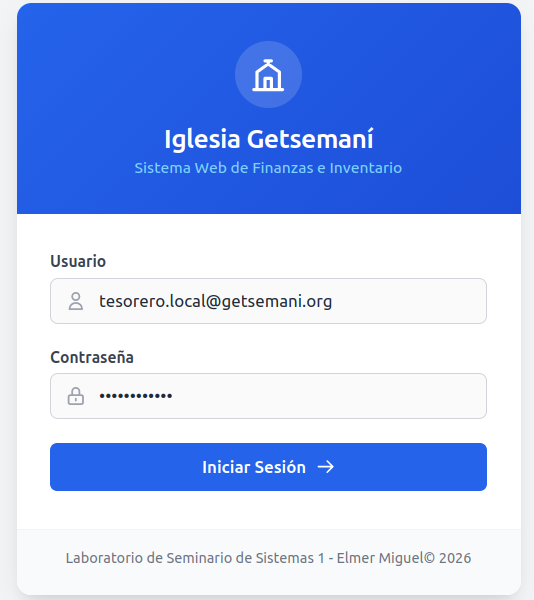
\includegraphics[width=0.7\linewidth]{img/1}
		\caption{Login}
		\label{fig:1}
	\end{figure}
	\newpage
	
	
	\begin{landscape}
		
	\begin{figure}
		\centering
		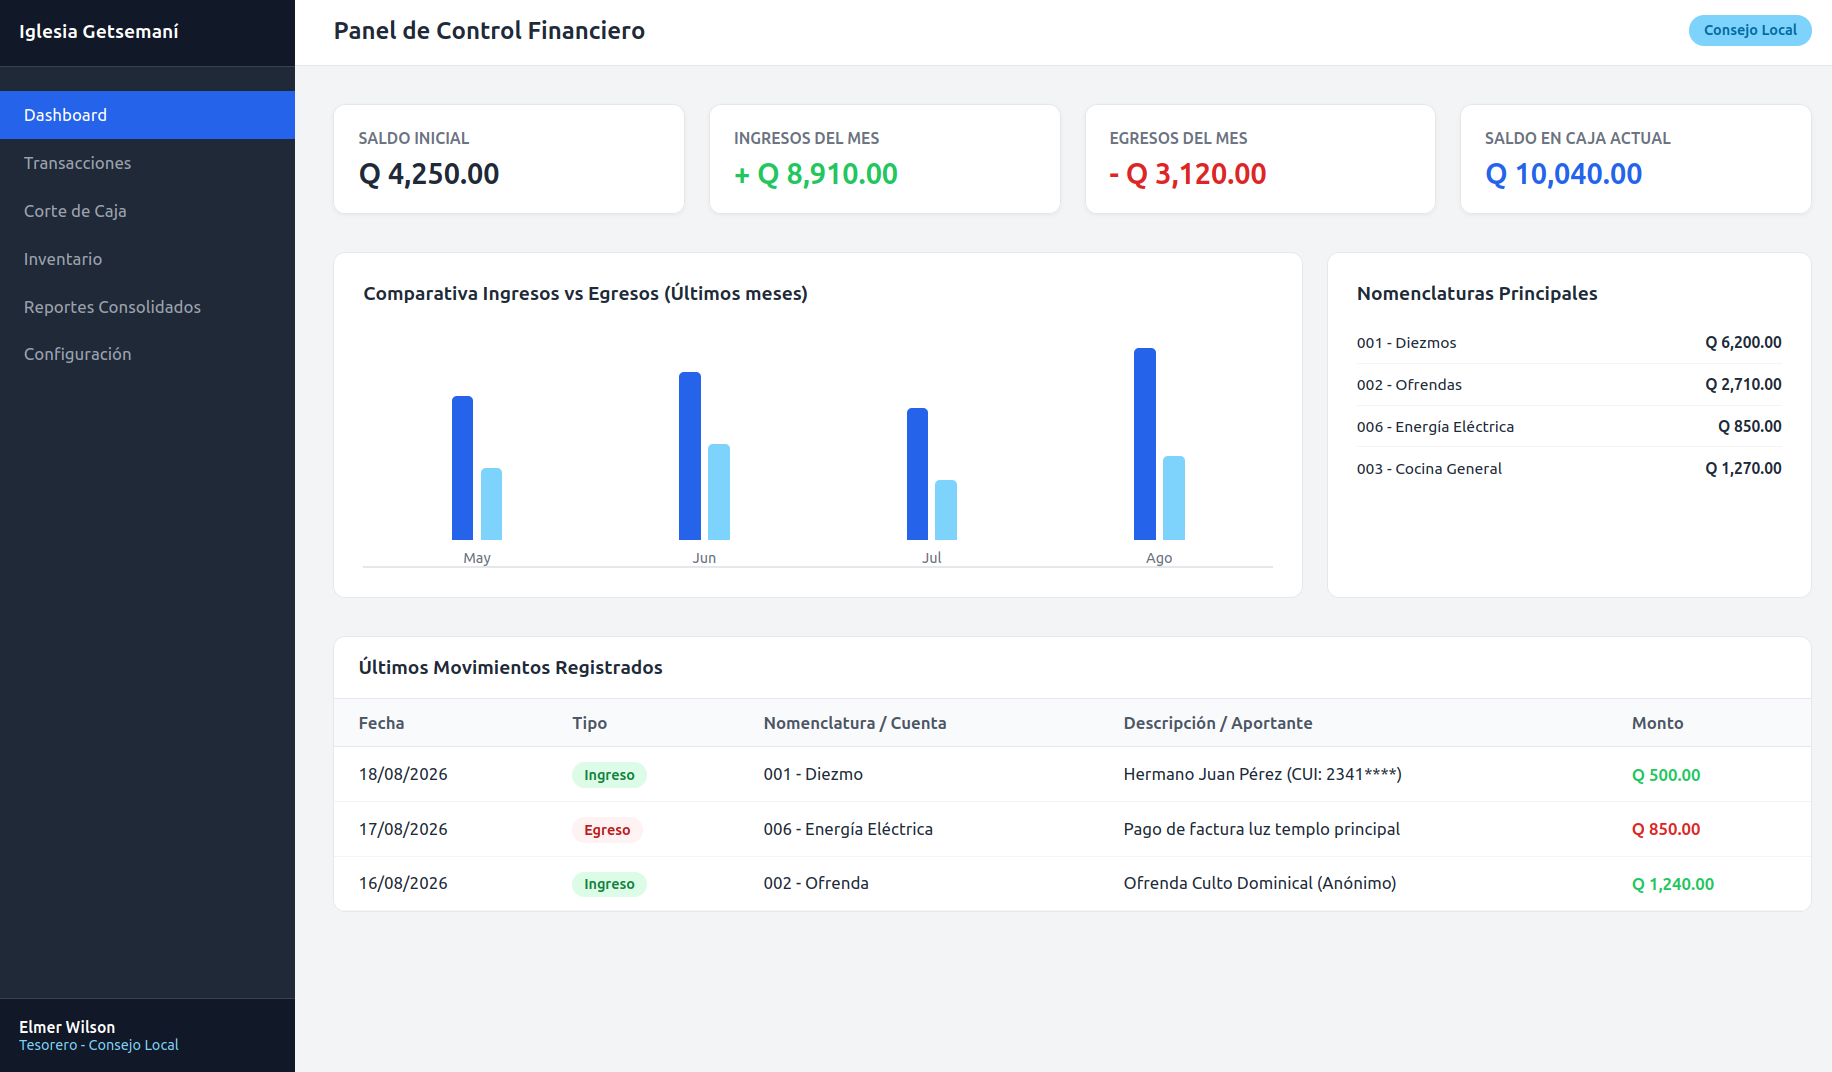
\includegraphics[width=1\linewidth]{img/2}
		\caption{Dashboard}
		\label{fig:2}
	\end{figure}
	
	\newpage
	\begin{figure}
		\centering
		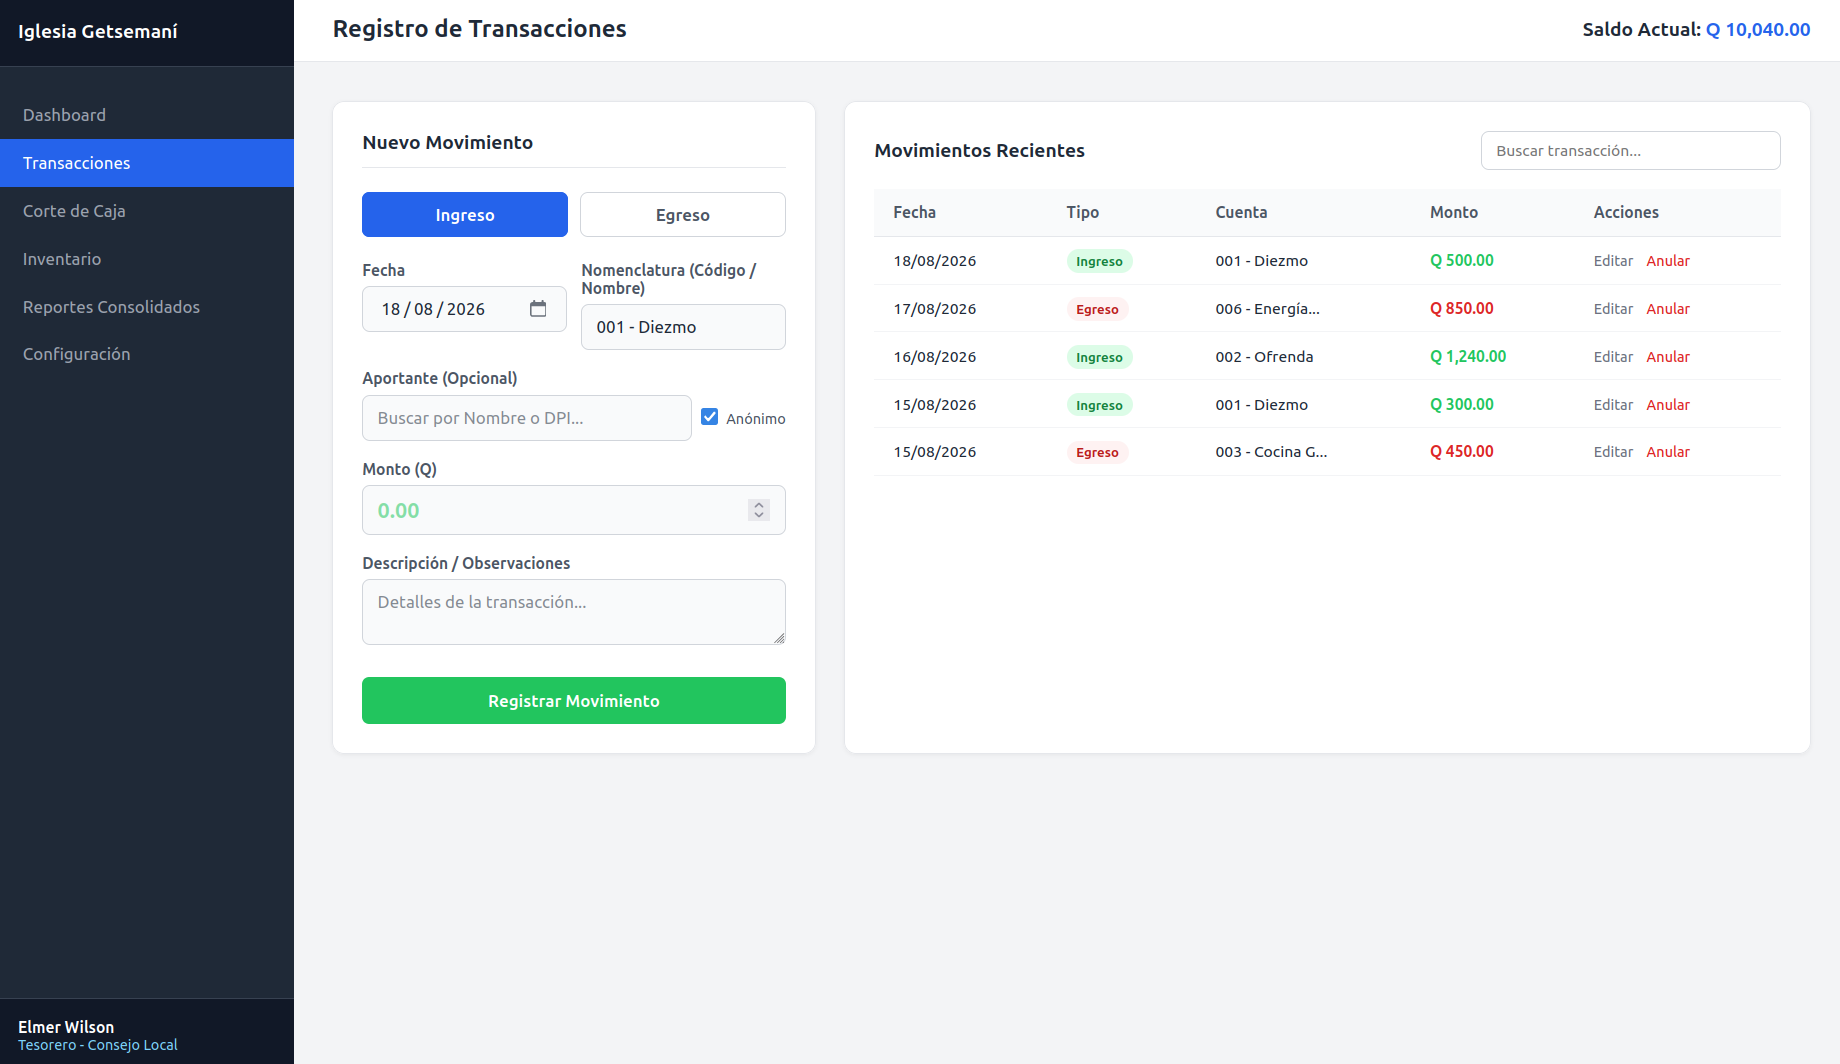
\includegraphics[width=1\linewidth]{img/3}
		\caption{Registro de Transacciones}
		\label{fig:3}
	\end{figure}
	
	
	
	
	\end{landscape}
	
	
\end{document}